% Draft captions written by C2_evaluation*.ipynb (knn). Overwritten on rerun.

% knn_aim0_msp_variants
\begin{figure}[t]
  \centering
  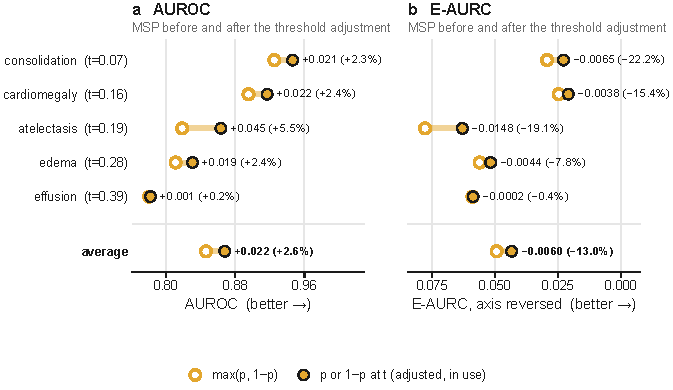
\includegraphics[width=\textwidth]{figures/c2/knn_aim0_msp_variants.pdf}
  \caption{Choice of the MSP baseline. Mean-fold AUROC (a, higher is better) and E-AURC (b, lower is better) of the plain $\max(p, 1-p)$ (hollow) and of the probability of the class C0 predicts at its Youden threshold $t$ (filled, the baseline used throughout), per task, ordered by C0's Youden threshold $t$, and their average. The line is what moving the decision boundary from 0.5 to $t$ changes; the gain is printed beside it (AUROC increase in a, E-AURC reduction in b, so positive is better in both).}
  \label{fig:knn_aim0_msp_variants}
\end{figure}

% knn_aim1a_attr_k_sweep
\begin{figure}[t]
  \centering
  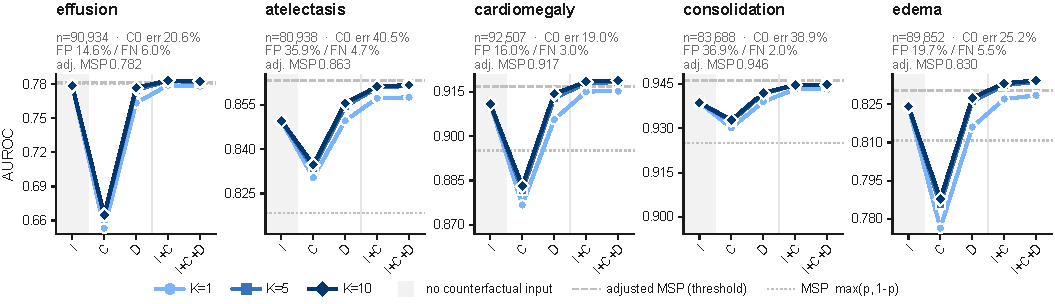
\includegraphics[width=\textwidth]{figures/c2/knn_aim1a_attr_k_sweep.pdf}
  \caption{Attribute models: mean-fold AUROC of every input configuration, one line per number of counterfactual neighbours $K \in \{1, 5, 10\}$. I: query attributes; C: counterfactual attributes; D: query minus counterfactual. The shaded configuration (I) sees no counterfactual, so its lines coincide across $K$. Grey lines: threshold-adjusted MSP (dashed) and plain $\max(p, 1-p)$ (dotted), the untrained baselines. Each panel has its own $y$-range.}
  \label{fig:knn_aim1a_attr_k_sweep}
\end{figure}

% knn_aim1c_cnn_k_sweep
\begin{figure}[t]
  \centering
  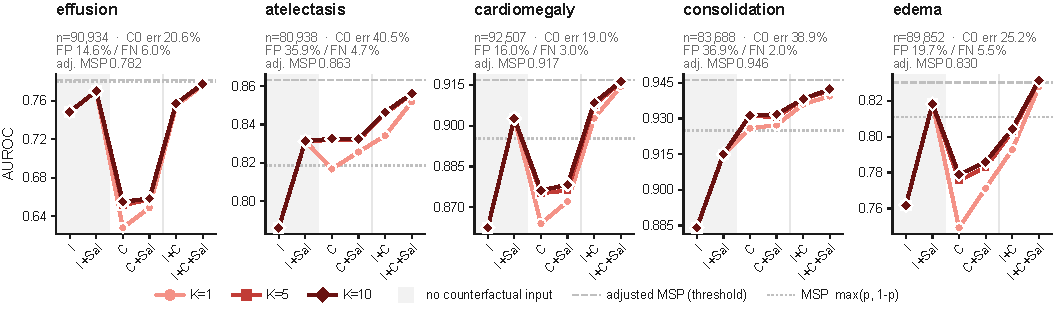
\includegraphics[width=\textwidth]{figures/c2/knn_aim1c_cnn_k_sweep.pdf}
  \caption{Image models: mean-fold AUROC of every CNN variant, one line per $K \in \{1, 5, 10\}$. I: query image; C: counterfactual image; Sal: saliency maps; I+C uses one encoder per image. The shaded models see no counterfactual, so their lines coincide across $K$. Grey lines: threshold-adjusted MSP (dashed) and plain $\max(p, 1-p)$ (dotted), the untrained baselines. Each panel has its own $y$-range.}
  \label{fig:knn_aim1c_cnn_k_sweep}
\end{figure}

% knn_aim1d_attr_blocks_bars
\begin{figure}[t]
  \centering
  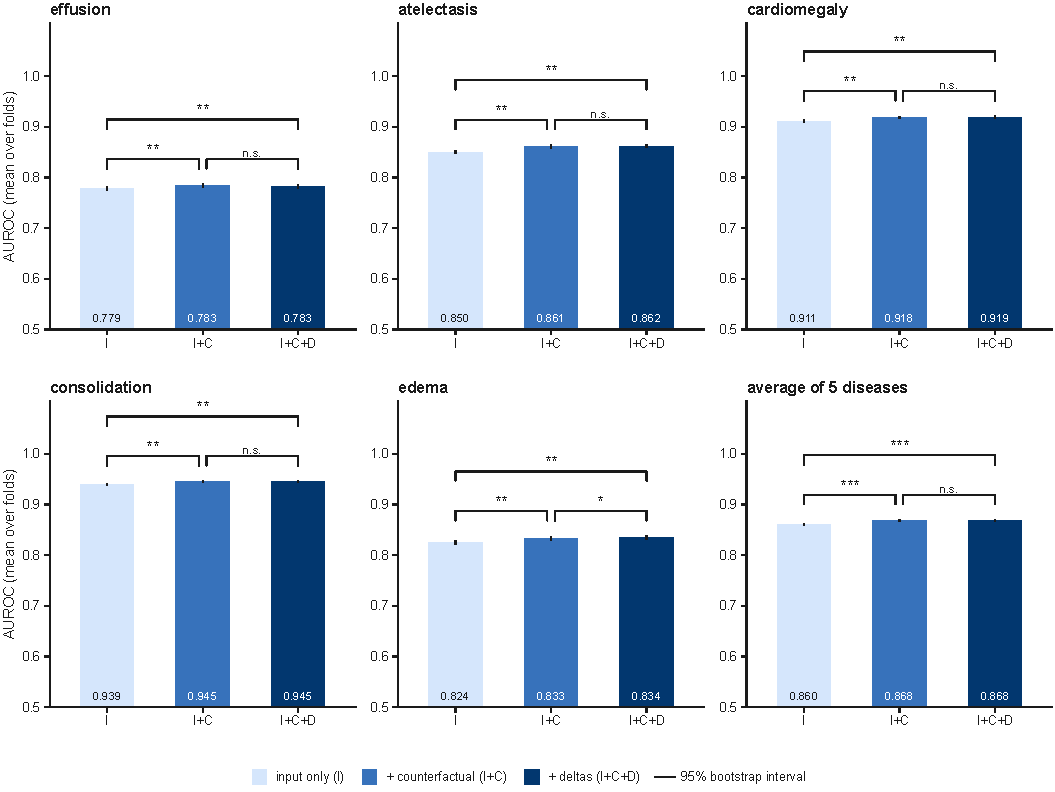
\includegraphics[width=\textwidth]{figures/c2/knn_aim1d_attr_blocks_bars.pdf}
  \caption{Adding the counterfactual to the attribute model, at $K = 10$. Bars: mean-fold AUROC of the query alone (I), with the counterfactual (I+C) and with the explicit deltas (I+C+D); whiskers: 95\% bootstrap interval of each AUROC. Brackets: paired patient-level bootstrap (5{,}000 replicates) of the mean-fold AUROC difference, Holm-adjusted across the 5 diseases (disease panels) or across the 9 claims (average panel); ***~$p_\mathrm{adj} < 0.001$, **~$p_\mathrm{adj} < 0.01$, *~$p_\mathrm{adj} < 0.05$, n.s.\ otherwise. Both models are scored on the same patients, so overlapping whiskers do not imply a non-significant difference. Grey lines: threshold-adjusted MSP (dashed) and plain $\max(p, 1-p)$ (dotted), the untrained baselines.}
  \label{fig:knn_aim1d_attr_blocks_bars}
\end{figure}

% knn_aim1e_cnn_ladder_bars
\begin{figure}[t]
  \centering
  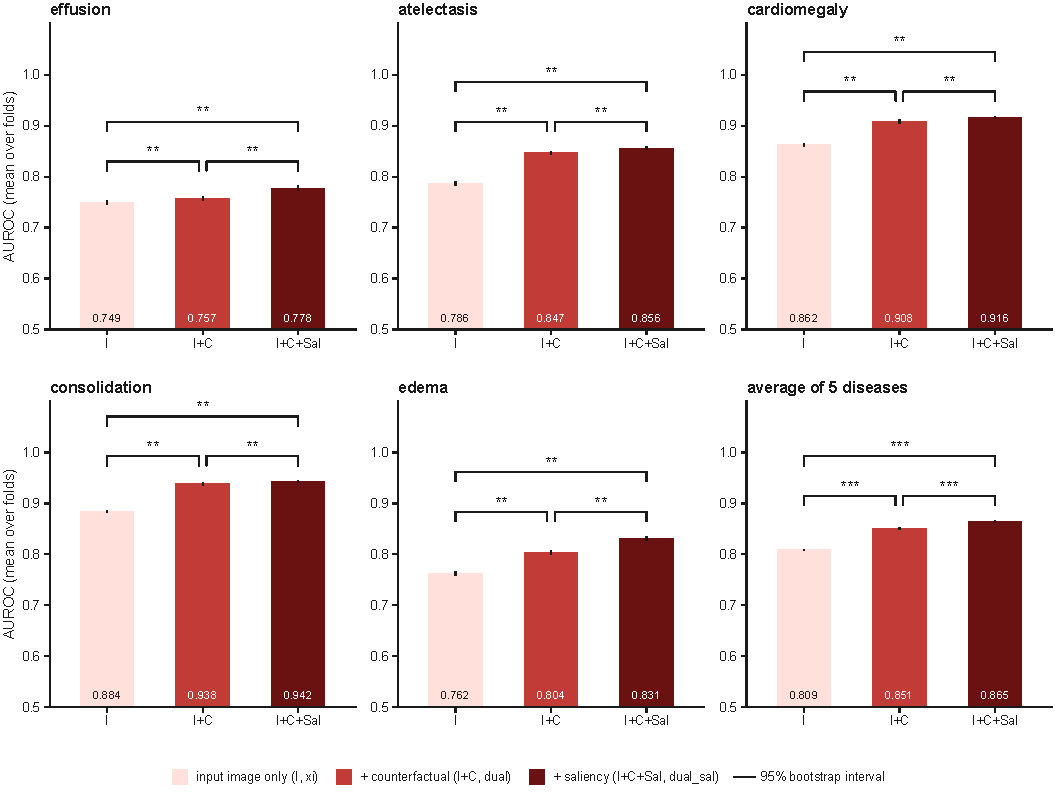
\includegraphics[width=\textwidth]{figures/c2/knn_aim1e_cnn_ladder_bars.pdf}
  \caption{Adding the counterfactual to the image model, at $K = 10$. Bars: mean-fold AUROC of the query image alone (I), with the counterfactual through a second encoder (I+C) and with both saliency maps (I+C+Sal); whiskers: 95\% bootstrap interval of each AUROC. Brackets: paired patient-level bootstrap (5{,}000 replicates) of the mean-fold AUROC difference, Holm-adjusted across the 5 diseases (disease panels) or across the 9 claims (average panel); ***~$p_\mathrm{adj} < 0.001$, **~$p_\mathrm{adj} < 0.01$, *~$p_\mathrm{adj} < 0.05$, n.s.\ otherwise. Grey lines: threshold-adjusted MSP (dashed) and plain $\max(p, 1-p)$ (dotted), the untrained baselines.}
  \label{fig:knn_aim1e_cnn_ladder_bars}
\end{figure}

% knn_aim1f_prob_bars
\begin{figure}[t]
  \centering
  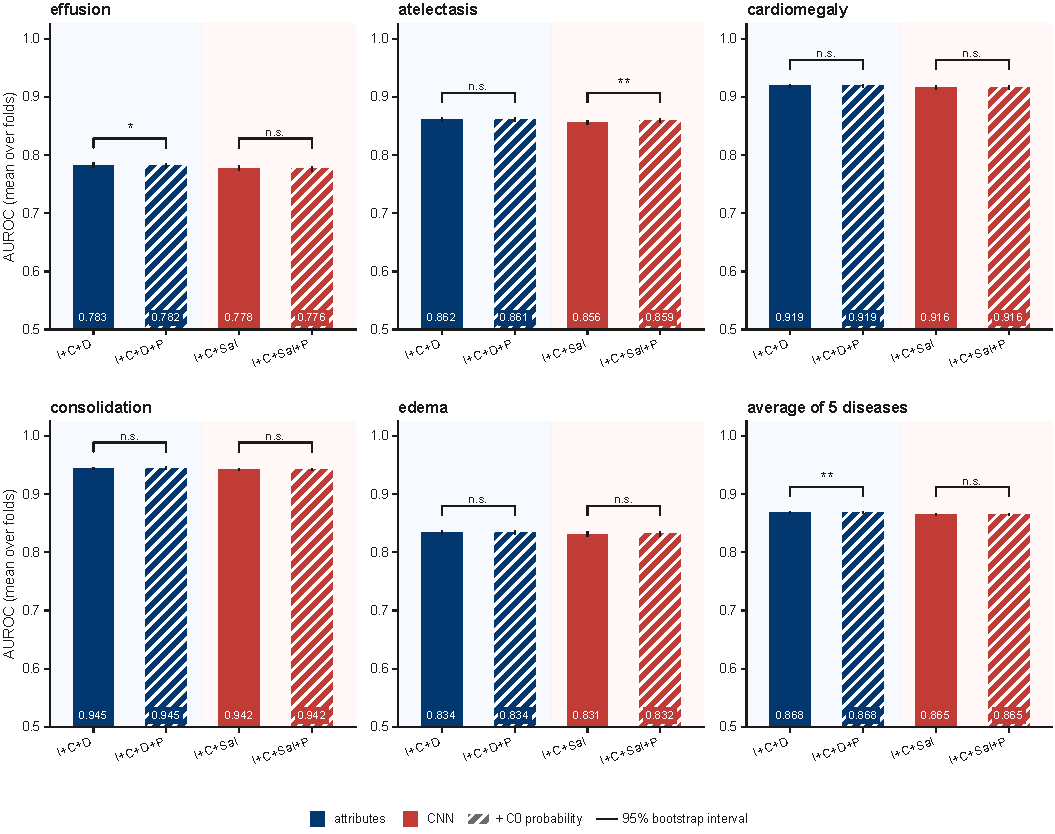
\includegraphics[width=\textwidth]{figures/c2/knn_aim1f_prob_bars.pdf}
  \caption{Adding C0's probability to each family's final model, at $K = 10$: the attribute model (I+C+D) and the CNN (I+C+Sal), without and with (hatched) five probability scalars --- $p$ and its entropy for the query and the counterfactual, and their difference. Whiskers: 95\% bootstrap interval of each AUROC. Brackets: paired patient-level bootstrap (5{,}000 replicates) of the mean-fold AUROC difference, Holm-adjusted across the 5 diseases (disease panels) or across the two families (average panel); ***~$p_\mathrm{adj} < 0.001$, **~$p_\mathrm{adj} < 0.01$, *~$p_\mathrm{adj} < 0.05$, n.s.\ otherwise. Grey lines: threshold-adjusted MSP (dashed) and plain $\max(p, 1-p)$ (dotted), the untrained baselines.}
  \label{fig:knn_aim1f_prob_bars}
\end{figure}

% knn_aim2a_best_vs_msp
\begin{figure}[t]
  \centering
  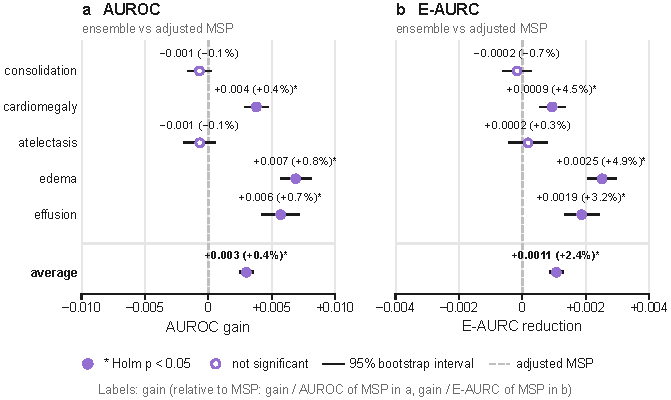
\includegraphics[width=\textwidth]{figures/c2/knn_aim2a_best_vs_msp.pdf}
  \caption{Final system against the adjusted MSP, at $K = 10$. Gain of the final system's strongest model (the ensemble in every disease) over the probability of the class C0 predicts at its Youden threshold $t$, in mean-fold AUROC (a) and mean-fold E-AURC (b, MSP minus model, so positive is better); the dashed line is the MSP. Tasks are ordered by C0's threshold. Each label gives the gain and, in brackets, the gain relative to MSP's score: $\mathrm{gain}/\mathrm{AUROC}_\mathrm{MSP}$ in (a) and $\mathrm{gain}/\mathrm{E\text{-}AURC}_\mathrm{MSP}$ in (b). The average row gives the mean gain and the mean of the five per-task percentages. Whiskers: 95\% intervals of a paired patient-level bootstrap (5{,}000 replicates). Filled points and $*$: Holm-adjusted $p < 0.05$. The correction runs across the 5 tasks within each panel, separately for (a) and (b), not across all 10 tests; the AUROC average is corrected across the 9 thesis claims, the E-AURC average is a single test.}
  \label{fig:knn_aim2a_best_vs_msp}
\end{figure}

% knn_aim2a_risk_coverage
\begin{figure}[t]
  \centering
  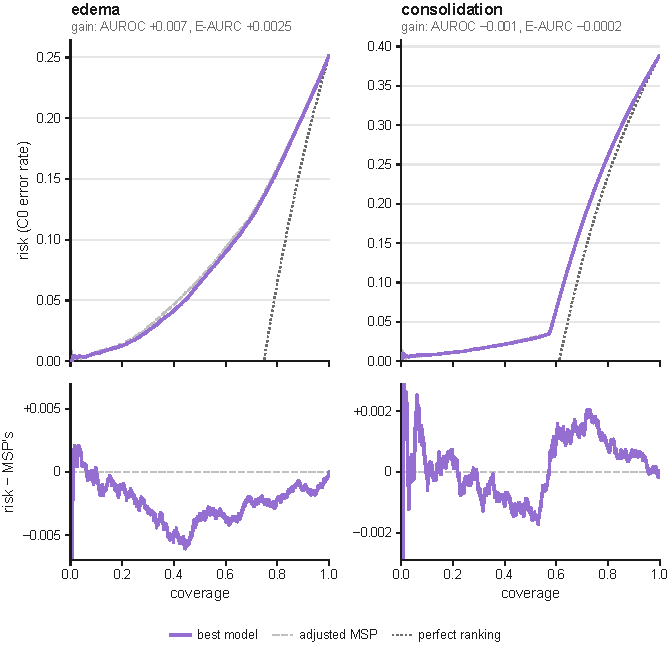
\includegraphics[width=\textwidth]{figures/c2/knn_aim2a_risk_coverage.pdf}
  \caption{Risk-coverage of the final system's strongest model against the adjusted MSP, for the tasks with the largest and smallest AUROC gain. Top: C0's error rate among the retained cases, most confident first; dotted: a perfect ranking. Bottom: the model's risk minus MSP's (below zero: fewer errors retained). Pooled out-of-fold predictions; the first 200 retained cases are not drawn.}
  \label{fig:knn_aim2a_risk_coverage}
\end{figure}

% knn_aim2b_ensemble
\begin{figure}[t]
  \centering
  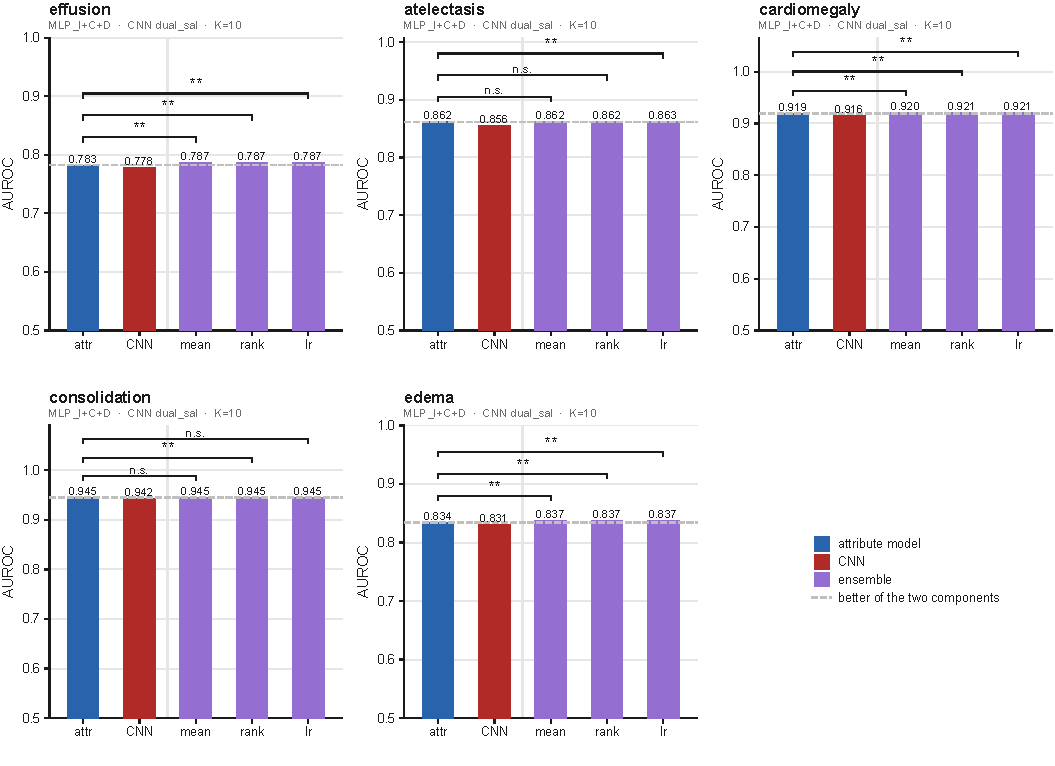
\includegraphics[width=\textwidth]{figures/c2/knn_aim2b_ensemble.pdf}
  \caption{Combining the final attribute model and CNN ($K = 10$). Bars: mean-fold AUROC of the two components and three combiners --- the mean of the two probabilities, the mean of their within-fold ranks, and a logistic regression fitted leave-one-fold-out. Dashed line: the better component. Brackets: paired patient-level bootstrap (5{,}000 replicates) of the mean-fold AUROC difference, Holm-adjusted across the 15 combiner--disease tests of the figure, of each combiner against the better component; ***~$p_\mathrm{adj} < 0.001$, **~$p_\mathrm{adj} < 0.01$, *~$p_\mathrm{adj} < 0.05$, n.s.\ otherwise.}
  \label{fig:knn_aim2b_ensemble}
\end{figure}

% knn_aim2d_baselines
\begin{figure}[t]
  \centering
  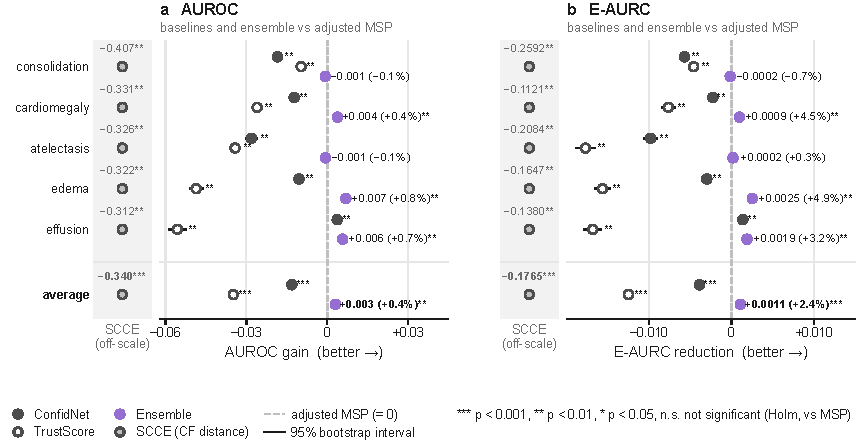
\includegraphics[width=\textwidth]{figures/c2/knn_aim2d_baselines.pdf}
  \caption{The final system and three prior-art failure predictors against the adjusted MSP, at $K = 10$: ConfidNet (filled), an MLP on C0's frozen penultimate features trained to regress the threshold-adapted true-class probability; TrustScore (open), the ratio of the distances to the nearest training points of the other and the predicted class; and SCCE, the distance to the nearest of the ensemble's own counterfactuals in the retrieval's attribute space. Gain over the probability of the class C0 predicts at its Youden threshold $t$ in mean-fold AUROC (a) and mean-fold E-AURC (b, MSP minus model), so right of the dashed line is better; tasks ordered by C0's threshold. SCCE is an order of magnitude further from MSP than the other methods and is shown in a strip of its own left of each panel, with its gain. The ensemble's gain is printed beside it. Whiskers: 95\% intervals of a paired patient-level bootstrap (5{,}000 replicates). $*$: Holm-adjusted $p < 0.05$ against the MSP, across the 5 tasks within each method and panel; the average row is a single test.}
  \label{fig:knn_aim2d_baselines}
\end{figure}

% knn_aim1d_attr_blocks_points
\begin{figure}[t]
  \centering
  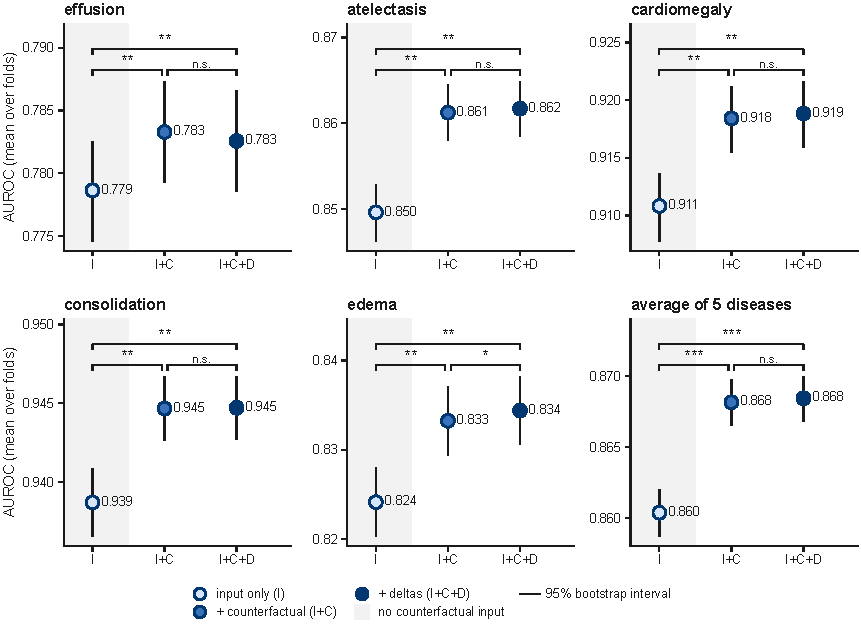
\includegraphics[width=\textwidth]{figures/c2/knn_aim1d_attr_blocks_points.pdf}
  \caption{Adding the counterfactual to the attribute model, at $K = 10$. Points: mean-fold AUROC of the query alone (I), with the counterfactual (I+C) and with the explicit deltas (I+C+D); whiskers: 95\% bootstrap interval of each AUROC. Brackets: paired patient-level bootstrap (5{,}000 replicates) of the mean-fold AUROC difference, Holm-adjusted across the 5 diseases (disease panels) or across the 9 claims (average panel); ***~$p_\mathrm{adj} < 0.001$, **~$p_\mathrm{adj} < 0.01$, *~$p_\mathrm{adj} < 0.05$, n.s.\ otherwise. Both models are scored on the same patients, so overlapping whiskers do not imply a non-significant difference. Grey lines: threshold-adjusted MSP (dashed) and plain $\max(p, 1-p)$ (dotted), the untrained baselines. Each panel has its own $y$-range, so compare models within a panel, not heights across panels; an MSP outside the range is printed in the panel corner.}
  \label{fig:knn_aim1d_attr_blocks_points}
\end{figure}

% knn_aim1e_cnn_ladder_points
\begin{figure}[t]
  \centering
  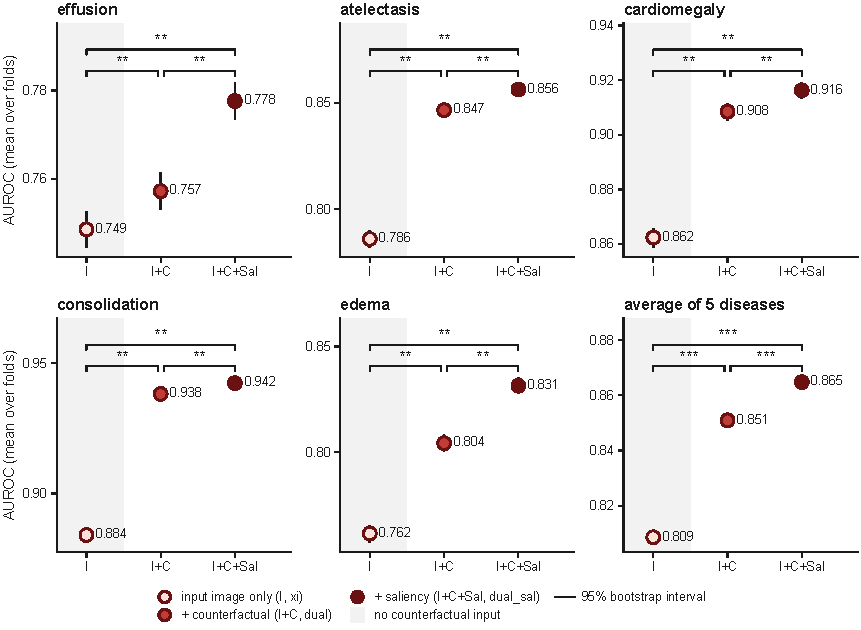
\includegraphics[width=\textwidth]{figures/c2/knn_aim1e_cnn_ladder_points.pdf}
  \caption{Adding the counterfactual to the image model, at $K = 10$. Points: mean-fold AUROC of the query image alone (I), with the counterfactual through a second encoder (I+C) and with both saliency maps (I+C+Sal); whiskers: 95\% bootstrap interval of each AUROC. Brackets: paired patient-level bootstrap (5{,}000 replicates) of the mean-fold AUROC difference, Holm-adjusted across the 5 diseases (disease panels) or across the 9 claims (average panel); ***~$p_\mathrm{adj} < 0.001$, **~$p_\mathrm{adj} < 0.01$, *~$p_\mathrm{adj} < 0.05$, n.s.\ otherwise. Grey lines: threshold-adjusted MSP (dashed) and plain $\max(p, 1-p)$ (dotted), the untrained baselines. Each panel has its own $y$-range, so compare models within a panel, not heights across panels; an MSP outside the range is printed in the panel corner.}
  \label{fig:knn_aim1e_cnn_ladder_points}
\end{figure}

% knn_aim1f_prob_points
\begin{figure}[t]
  \centering
  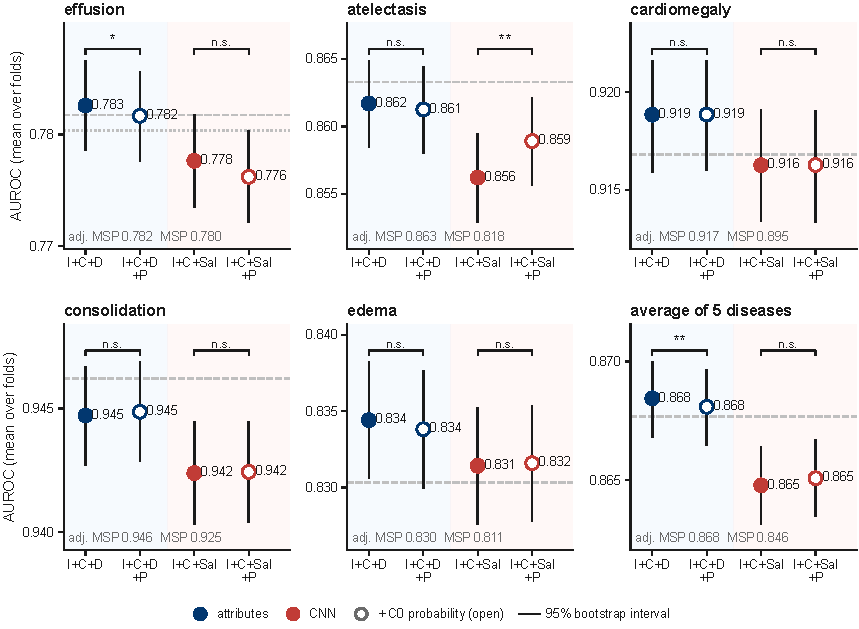
\includegraphics[width=\textwidth]{figures/c2/knn_aim1f_prob_points.pdf}
  \caption{Adding C0's probability to each family's final model, at $K = 10$: the attribute model (I+C+D) and the CNN (I+C+Sal), without and with (open points) five probability scalars --- $p$ and its entropy for the query and the counterfactual, and their difference. Whiskers: 95\% bootstrap interval of each AUROC. Brackets: paired patient-level bootstrap (5{,}000 replicates) of the mean-fold AUROC difference, Holm-adjusted across the 5 diseases (disease panels) or across the two families (average panel); ***~$p_\mathrm{adj} < 0.001$, **~$p_\mathrm{adj} < 0.01$, *~$p_\mathrm{adj} < 0.05$, n.s.\ otherwise. Grey lines: threshold-adjusted MSP (dashed) and plain $\max(p, 1-p)$ (dotted), the untrained baselines. Each panel has its own $y$-range, so compare models within a panel, not heights across panels; an MSP outside the range is printed in the panel corner.}
  \label{fig:knn_aim1f_prob_points}
\end{figure}

% knn_aim2b_ensemble_points
\begin{figure}[t]
  \centering
  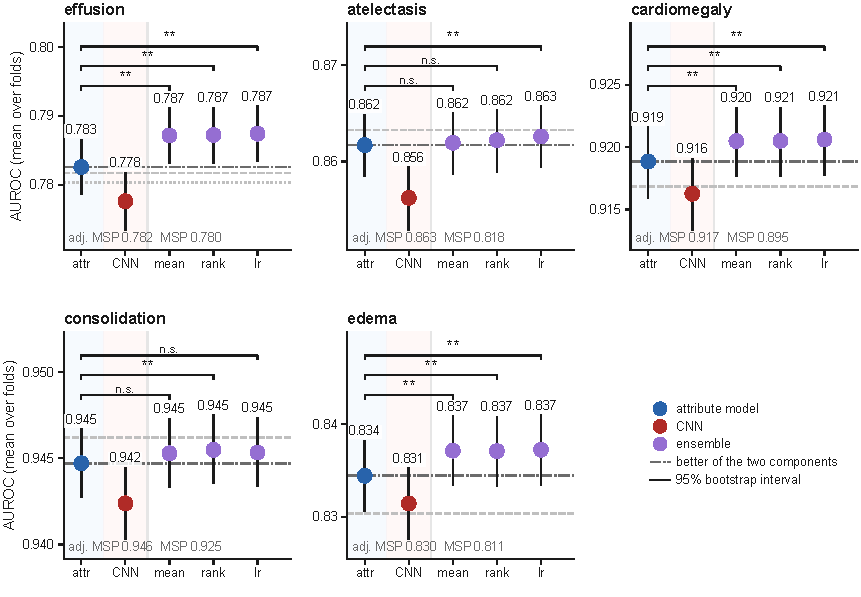
\includegraphics[width=\textwidth]{figures/c2/knn_aim2b_ensemble_points.pdf}
  \caption{Combining the final attribute model and CNN ($K = 10$). Points: mean-fold AUROC of the two components and three combiners --- the mean of the two probabilities, the mean of their within-fold ranks, and a logistic regression fitted leave-one-fold-out. Whiskers: 95\% bootstrap interval. Dash-dotted line: the better component; grey dashed and dotted lines: threshold-adjusted MSP and $\max(p, 1-p)$. Brackets: paired patient-level bootstrap (5{,}000 replicates) of the mean-fold AUROC difference, Holm-adjusted across the 15 combiner--disease tests of the figure, of each combiner against the better component; ***~$p_\mathrm{adj} < 0.001$, **~$p_\mathrm{adj} < 0.01$, *~$p_\mathrm{adj} < 0.05$, n.s.\ otherwise. Each panel has its own $y$-range, so compare models within a panel, not heights across panels; an MSP outside the range is printed in the panel corner.}
  \label{fig:knn_aim2b_ensemble_points}
\end{figure}
